\section{Searching}
Figure \ref{fig:homepage} shows the homepage for DSPLearn, which features a search bar.

\begin{figure}[!htbp]
  \centering
  
\includegraphics[width=\textwidth]{system_demonstration/demo_homepage.jpg}
  \caption{DSPLearn Homepage}
  \label{fig:homepage}
\end{figure}

When a query is entered, the browser would be directed to the result page (Figure \ref{fig:result_page}). As seen, users can also enter new queries in the search bar on top of the result page. The left sidebar features a hierarchical concept tree. The tree consists of concepts that are related to one or more documents in the search results. The blue badge near each concept indicates the number of documents in the search results that are related to the concept. The total number of search results is shown in the green notification bar. The section title, the book the section is in, and the excerpt are displayed for each document in the search results. The excerpt has a maximum of 500 characters and the keywords from the query are in bold. Those \texttt{...} placeholders are replacement of \texttt{[FORMULA]} from the document text.

\begin{figure}[!htbp]
  \centering
  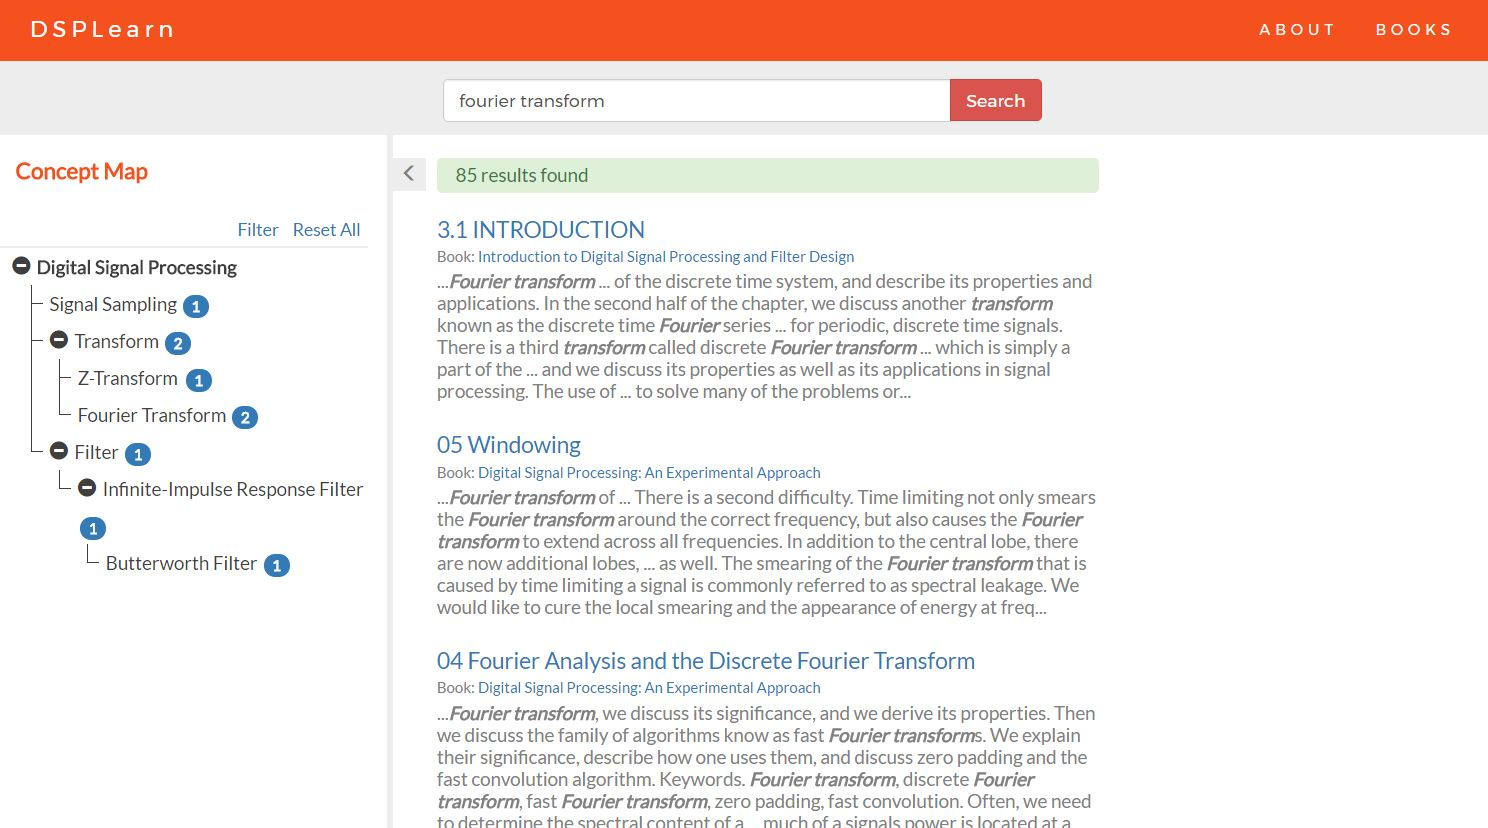
\includegraphics[width=\textwidth]{system_demonstration/demo_result_page.jpg}
  \caption{DSPLearn Page for Search Results}
  \label{fig:result_page}
\end{figure}

The search results are paginated (Figure \ref{fig:result_paginate}). Each page contains 10 search results. Users may navigate to the previous or the next page via the buttons at the bottom of the page. They may also slide the page to the top by selecting the arrow button on the bottom right.

\begin{figure}[!htbp]
  \centering
  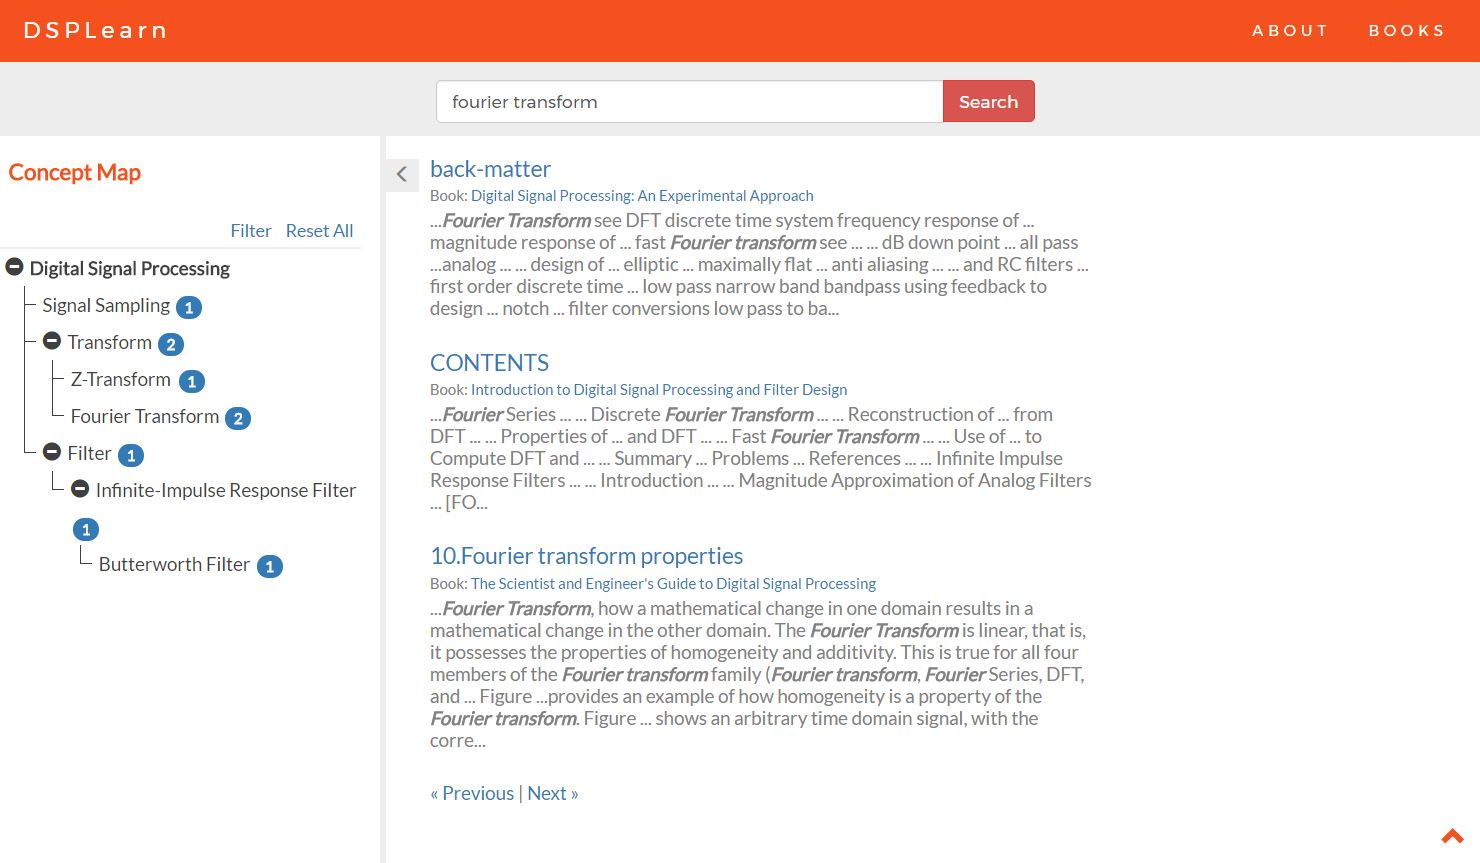
\includegraphics[width=\textwidth]{system_demonstration/demo_result_pagination.jpg}
  \caption{Pagination of Search Results}
  \label{fig:result_paginate}
\end{figure}

The concept tree on the sidebar is interactive. A dialog would pop up when users select a concept (Figure \ref{fig:result_popover}). Users may set the filtering condition for each concept by selecting whether each document of the search results must or must not be related to the concept.

\begin{figure}[!htbp]
  \centering
  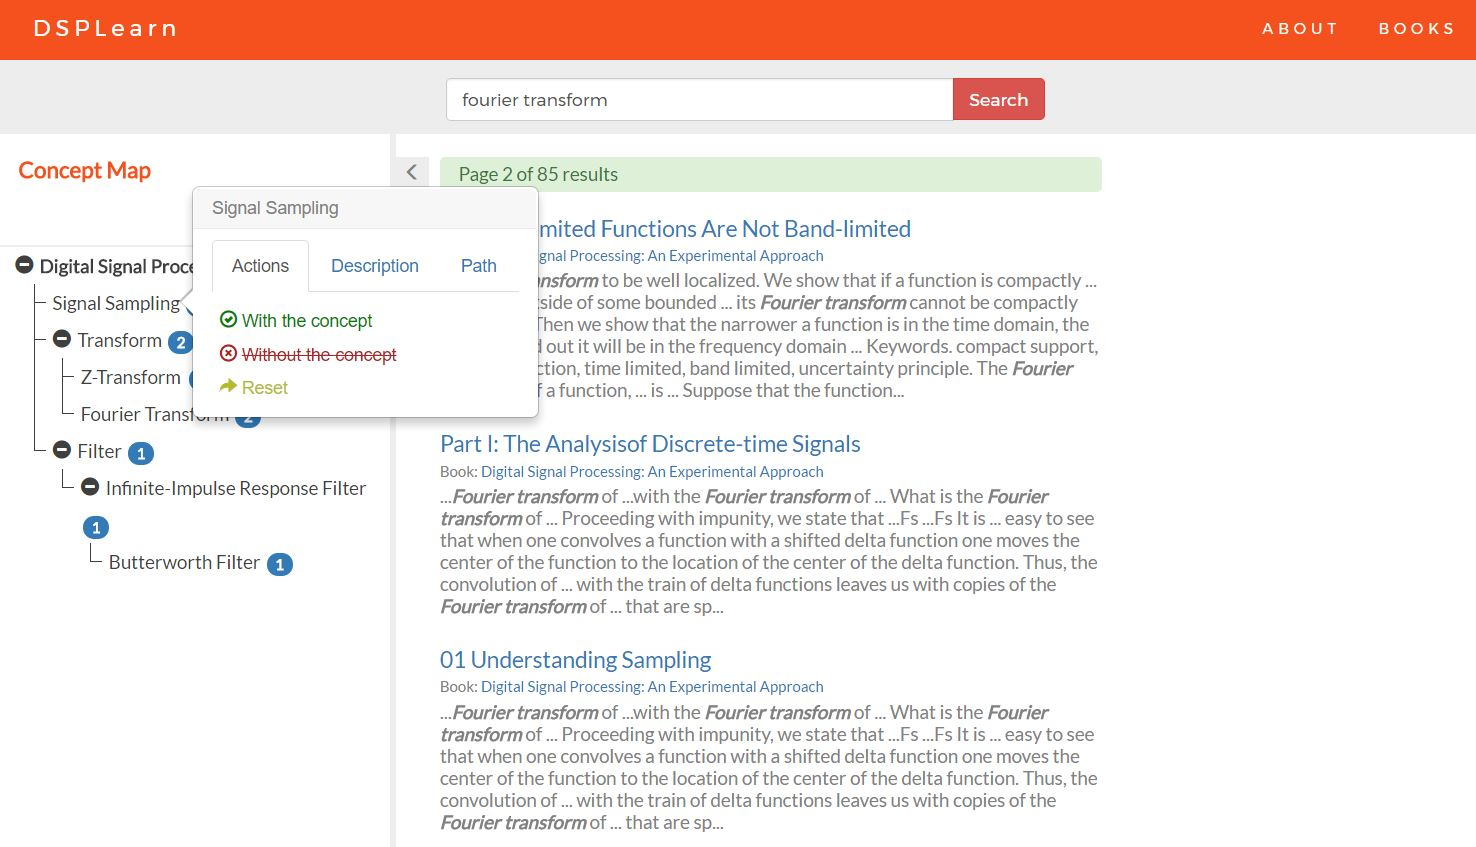
\includegraphics[width=\textwidth]{system_demonstration/demo_result_popover.jpg}
  \caption{Concept Popover in Result Page}
  \label{fig:result_popover}
\end{figure}

The dialog has 3 tabs - \enquote{Actions}, \enquote{Description}, and \enquote{Path}. The description of each tab is below.

\begin{itemize}
\item \textbf{Actions:} Choose an action to filter the search results - \enquote{With the concept}, \enquote{Without the concept}, or \enquote{Reset}
\item \textbf{Description:} Definition of the concept
\item \textbf{Path:} Concept path from the root concept node to the current node in the ontology
\end{itemize}

As seen in Figure \ref{fig:sfig:result_filter_before}, a concept would be in green if users select \enquote{With the concept} in the concept dialog and in red if users select \enquote{Without the concept} instead. Users may select \enquote{Reset} to impose no constraint on the search results for the concept.

When the \enquote{Filter} button is selected, DSPLearn would filter the search results based on the filtering conditions. Figure \ref{fig:sfig:result_filter_after} shows the results after the filtering is performed. As seen, the concept tree on the sidebar is also updated to reflect the new search results.

\begin{figure}[!htbp]
\centering
 
  \begin{subfigure}{\textwidth}
  \centering
  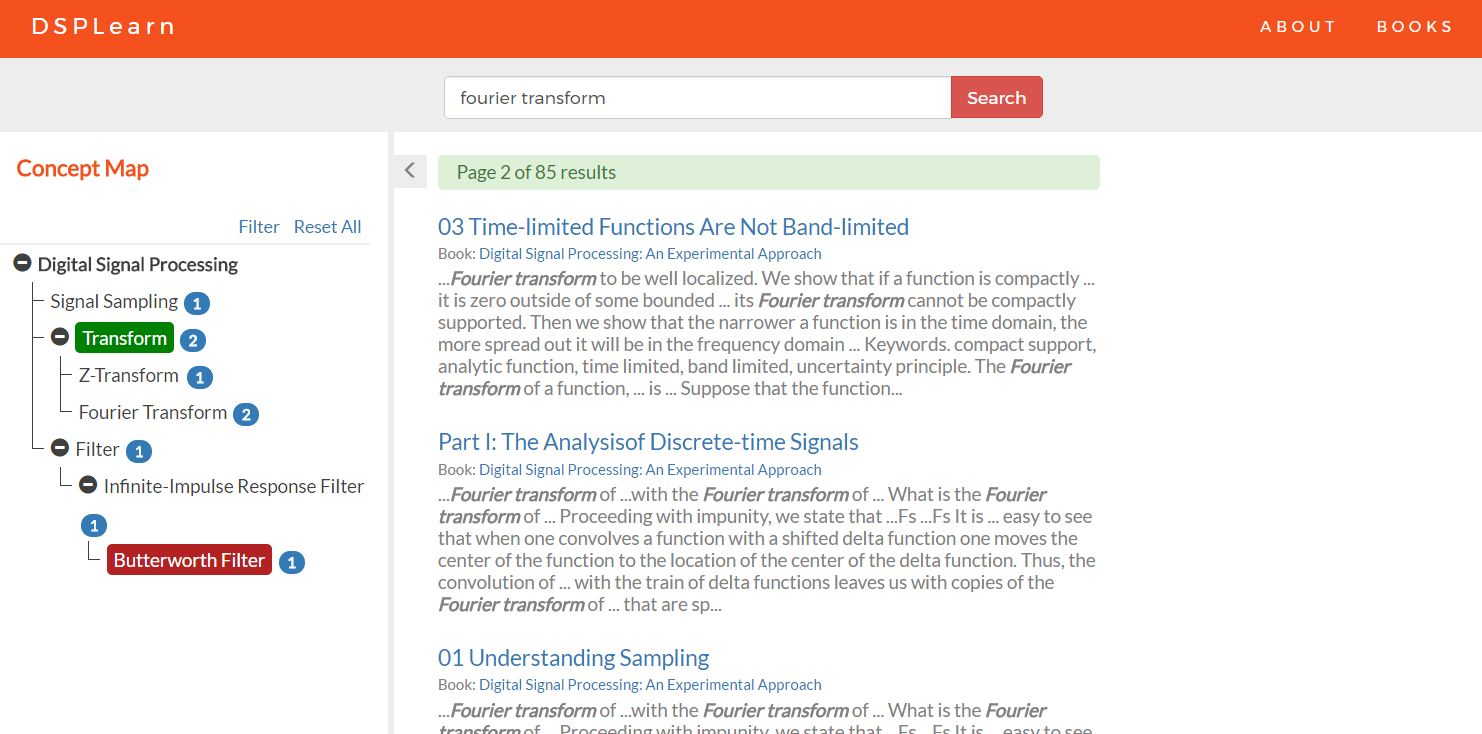
\includegraphics[width=\linewidth]{system_demonstration/demo_result_filter_before.jpg}
  \caption{Before Filtering}
  \label{fig:sfig:result_filter_before}
  \end{subfigure}
  
  \begin{subfigure}{\textwidth}
  \centering
  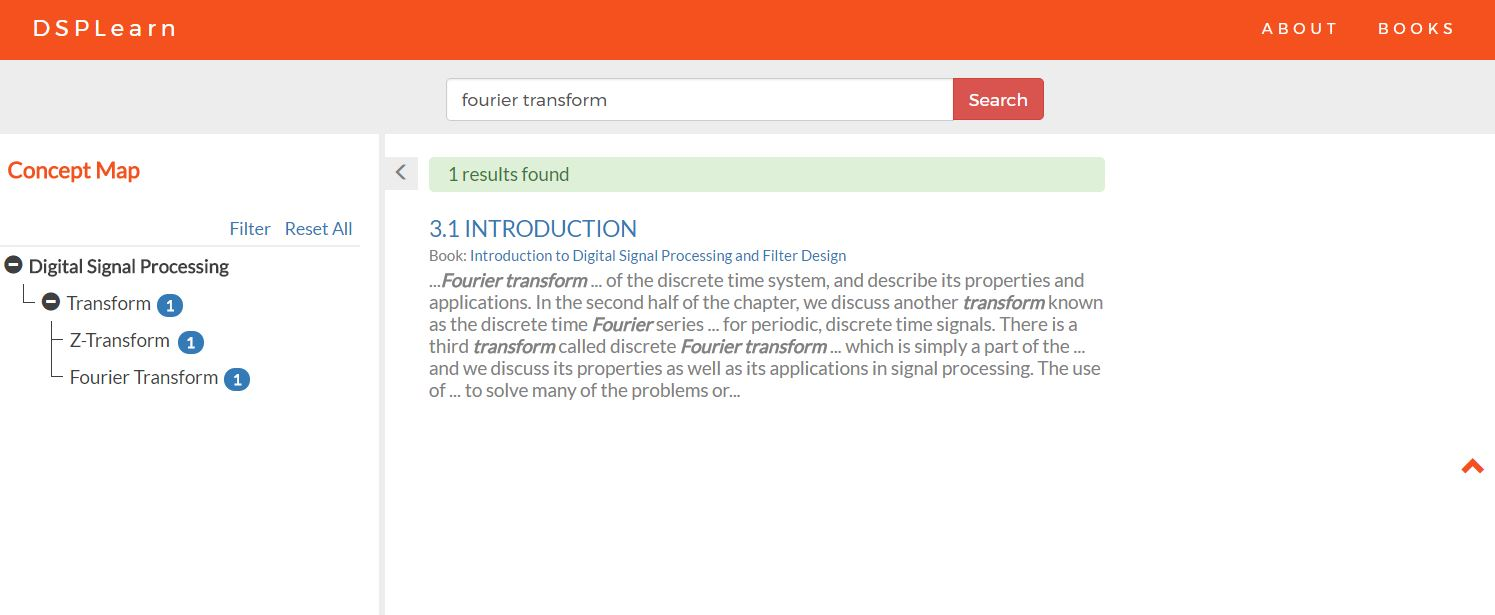
\includegraphics[width=\linewidth]{system_demonstration/demo_result_filter_after.jpg}
  \caption{After Filtering}
  \label{fig:sfig:result_filter_after}
  \end{subfigure}
 
\caption{Search Results Filtering}
\label{fig:result_filter}
\end{figure}


